\begin{figure}[h!]
    \centering
    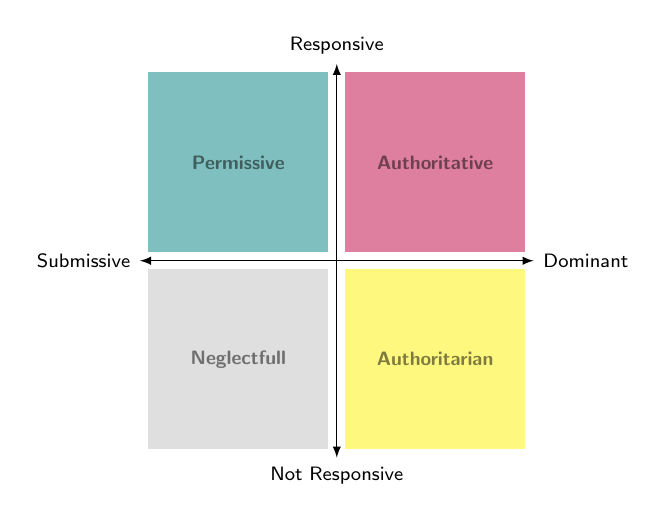
\begin{tikzpicture}[
            >=latex,
            scale=2.5,
            font=\sf\scriptsize,
            spacedots/.style={dotted, black, line width=0.5pt},
            stylerect/.style={rectangle, inner sep=0pt, minimum size = 65}
        ]
		\def\xaxis{1};
		\def\zaxis{1};
		\definecolor{myteal}{rgb}{1,0.5,0}
		\definecolor{mytomato}{rgb}{1,0.5,0}
		
		%Axes
		
		\draw[<->] (-\xaxis,0) -- (\xaxis,0) node[at end,right] { Dominant} node[at start,left] {Submissive};
		\draw[<->] (0,-\zaxis) -- (0,\zaxis) node[at end,above] {Responsive} node[at start,below] {Not Responsive};
		
		\node[stylerect,fill=teal, opacity=0.5] at (-0.5,0.5) {\textbf{Permissive}};
		\node[stylerect,fill=purple, opacity=0.5] at (0.5,0.5)  {\textbf{Authoritative}};
		
		
		\node[stylerect,fill=yellow, opacity=0.5] at (0.5,-0.5) {\textbf{Authoritarian}};
		\node[stylerect,fill=lightgray, opacity=0.5] at (-0.5,-0.5) {\textbf{Neglectfull}};
    \end{tikzpicture}
    \caption{Parenting Styles arranged on two axis as proposed by \cite{Darling1993}}

    \label{fig:fpareting_style}
\end{figure}